%!TEX root=../GaugeCNNTheory.tex


\subsection{ایزومتری‌ها و عمل آنها بر منیفلدها، کلاف‌ها و میدان‌ها}
\label{sec:isom_background}


\begin{figure}
    \centering
    \subcaptionbox{\small عمل زیرگروه‌های مختلف گروه ایزومتری بر روی میدان‌ها.
        \label{fig:isom_egg_actions}}%
        [.6\linewidth][l]{
            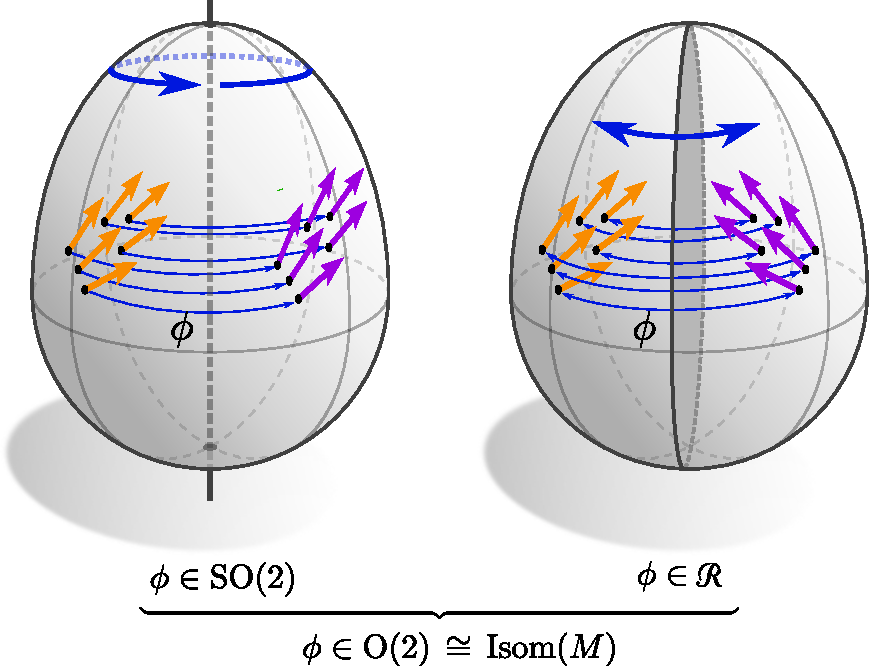
\includegraphics[width=.575\textwidth]{figures/isometry_egg_action.pdf}
        }
    \hfill
    \subcaptionbox{\small مدارهای گروه ایزومتری.
        \label{fig:isom_egg_orbits}}%
        [.3\linewidth][r]{
            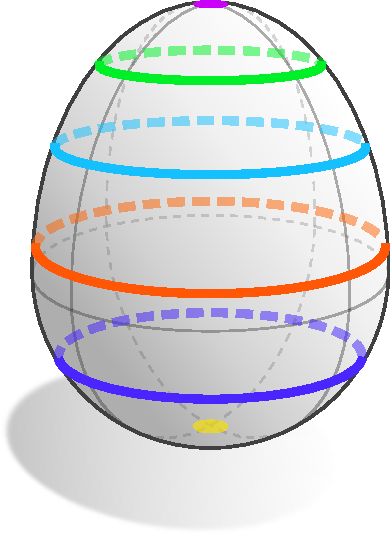
\includegraphics[width=.26\textwidth]{figures/isometry_egg_orbits.pdf}
            \hspace*{2ex}
            \vspace*{7.0ex}
        }
    \caption{\small
        تصاویری از گروه ایزومتری $\IsomM \cong \O2$ یک تخم‌مرغ $M$ که در سراسر این بخش برای نمونه‌سازی مفاهیم و ساختارهای مختلف مربوط به ایزومتری‌ها از آن استفاده خواهیم کرد.
        شکل~\ref{fig:isom_egg_actions} عمل گروه ایزومتری را بر روی میدان‌های برداری (مماس یا ویژگی) نشان می‌دهد.
        می‌توان آن را متشکل از زیرگروه‌های دوران‌ها در $\SO2$ و بازتاب‌ها در $\Flip$ در نظر گرفت.
        عمل گروه ایزومتری، تخم‌مرغ را به مدارهای $\IsomM.p = \big\{\phi(p) \,\big|\, \phi\in\IsomM\big\}$ از نقاط $p\in M$ افراز می‌کند که در شکل~\ref{fig:isom_egg_orbits} با رنگ‌های مختلف نشان داده شده‌اند.
        توجه داشته باشید که همه مدارها با یکدیگر همسان‌ریخت نیستند - مدارهای قطب‌ها نقاط منفرد هستند در حالی که هر مدار دیگر یک دایره را در اطراف تخم‌مرغ ترسیم می‌کند.
        گروه ایزومتری تخم‌مرغ به صورت غیرتعدی‌پذیر بر روی آن عمل می‌کند، یعنی نمی‌توان از هر نقطه‌ای به هر نقطه دیگر رسید.
        یک تبدیل میدان کرنل زمانی هم‌متغیر نسبت به ایزومتری است که با عمل ایزومتری بر روی میدان‌های ویژگی جابجا شود.
        ما نشان می‌دهیم که هم‌متغیری ایزومتری تنها و تنها در صورتی تضمین می‌شود که میدان کرنل تحت عمل ایزومتری‌ها نامتغیر باشد.
        این به طور خاص ایجاب می‌کند که هم‌متغیری ایزومتری نیازمند اشتراک‌گذاری وزن در امتداد مدارهای ایزومتری است؛ به شکل~\ref{fig:isom_invariant_kernel_field_multiple_orbits} مراجعه کنید.
    }
    \label{fig:isom_egg_main}
\end{figure}


در این بخش، ما بیشتر مفاهیم ریاضی مورد نیاز برای مطالعه هم‌متغیری ایزومتری تبدیلات میدان کرنل و کانولوشن‌های $\GM$ را معرفی می‌کنیم.
پس از تعریف ایزومتری‌ها در بخش~\ref{sec:isometry_groups}، در بخش~\ref{sec:isom_action_bundles} بحث می‌کنیم که چگونه آنها اعمال طبیعی را بر روی بردارهای مماس و قاب‌های مرجع القا می‌کنند.
برای گروه‌های ساختار $G<\O{d}$، هر ایزومتری با هر \lr{G}-ساختاری سازگار نیست.
ما زیرگروه $\IsomGM \leq \IsomM$ از آن ایزومتری‌هایی را تعریف می‌کنیم که بر روی یک \lr{G}-ساختار $\GM$ و کلاف‌های ویژگی \lr{G}-الحاقی آن عمل می‌کنند (خودریختی‌هایی را القا می‌کنند).
درحالی‌که این ساختارها مستقل از مختصات نگه داشته می‌شوند، بخش~\ref{sec:isom_coordinatization} عمل ایزومتری‌ها را بر روی کلاف‌های تاری نسبت به بدیهی‌سازی‌های محلی کلاف بیان می‌کند.
به عنوان مقدمه‌ای برای بررسی تبدیلات میدان کرنل هم‌متغیر نسبت به ایزومتری در ادامه، بخش~\ref{sec:isom_expmap_transport} بحث می‌کند که چگونه ایزومتری‌ها با نگاشت نمایی و با منتقل‌کننده‌های موازی جابجا می‌شوند، که به ما اجازه می‌دهد تا نحوه عمل ایزومتری‌ها را بر روی پول‌بک منتقل‌کننده $\Expspf$ میدان‌های ویژگی $f$ استخراج کنیم.
درحالی‌که عمدتاً ریاضی باقی می‌مانیم، سعی می‌کنیم تا حد امکان ارتباطاتی با کاربرد برقرار کنیم.


\subsubsection{گروه‌های ایزومتری}
\label{sec:isometry_groups}

یک \emph{ایزومتری} (سراسری) $\phi: M \to \hat{M}$ یک دیفئومورفیسم بین منیفلدهای ریمانی $(M,\eta)$ و $(\hat{M},\hat{\eta})$ است که \emph{متریک را حفظ می‌کند}.
بر حسب پیش‌ران (دیفرانسیل) $\dphiTM: \TM \to T\mkern-1.5mu\hat{M}$ بردارهای مماس، که در پیوست~\ref{apx:differentials_gradients_jacobians} و در بخش~\ref{sec:isom_action_bundles} در زیر معرفی می‌کنیم، این گزاره با الزام به اینکه ایزومتری‌ها برآورده کنند، دقیق می‌شود:
\begin{align}\label{eq:isometry_def}
    \eta_p(v,\, w)\ =\ \hat{\eta}_{\phi(p)}( \dphiTM v,\, \dphiTM w) \qquad \forall\ \ p\in M,\,\ v,w\in \TpM \,,
\end{align}
یعنی، آنها فاصله‌ها و زوایا بین بردارهای مماس را حفظ می‌کنند.
به طور شهودی، یک ایزومتری به عنوان یک نگاشت حافظ فاصله بین منیفلدها در نظر گرفته می‌شود.
توجه داشته باشید که معکوس یک ایزومتری لزوماً یک ایزومتری نیز هست.
از آنجایی که ایزومتری‌ها (و معکوس‌هایشان) به متریک احترام می‌گذارند، آنها \emph{ایزومورفیسم‌ها در رده منیفلدهای ریمانی} را تشکیل می‌دهند.


مجموعه تمام ایزومتری‌های $\phi: M \to M$ از یک منیفلد ریمانی به خودش، که با ترکیب معمول توابع $\circ: (\phi_1, \phi_2) \mapsto \phi_1 \circ \phi_2$ مجهز شده است، یک گروه را تعریف می‌کند که به عنوان \emph{گروه ایزومتری} $\IsomM$ از $M$ شناخته می‌شود.
این گروه، گروه خودریختی یک منیفلد ریمانی است که شامل تمام «تقارن‌های» (متریکی) آن است.
این یک زیرگروه از گروه دیفئومورفیسم $\Diff(M)$ از $M$ است.
گروه کامل ایزومتری ممکن است زیرگروه‌های غیربدیهی داشته باشد، که ما در ادامه با $\I \leq \IsomM$ نشان خواهیم داد.
یک مثال در شکل~\ref{fig:isom_egg_actions} آورده شده است، که گروه ایزومتری $\IsomM \cong \O2$ یک تخم‌مرغ را به تصویر می‌کشد.
گروه کامل ایزومتری (به عنوان مثال) به زیرگروه‌های دوران‌ها در $\I_1 \cong \SO2$ و بازتاب‌ها در $\I_2 \cong \Flip$ تقسیم می‌شود.


به طور کلی، گروه ایزومتری یک منیفلد غیرتعدی‌پذیر است، یعنی، هر نقطه‌ای از $M$ را نمی‌توان از هر نقطه دیگری با عمل آن رسید.
سپس منیفلد به \emph{مدارهای} مجزا افراز می‌شود که برای مثال $M$ به عنوان یک تخم‌مرغ (عید پاک) در شکل~\ref{fig:isom_egg_orbits} به تصویر کشیده شده است.
گروه ایزومتری یک منیفلد $M$ ممکن است بدیهی باشد، به شرطی که $M$ به اندازه کافی نامتقارن باشد.
در این حالت، ممکن است هنوز ایزومتری‌های غیربدیهی بین زیرمجموعه‌های باز $U^{\widetilde{A}}$ و $U^A$ از $M$ وجود داشته باشد، که معادله~\eqref{eq:isometry_def} به آنها محدود می‌شود.
شکل~\ref{fig:suzanne_local_isometry} نمونه‌ای از یک منیفلد را نشان می‌دهد که به صورت سراسری نامتقارن است اما ایزومتری‌های غیربدیهی بین زیرمجموعه‌های محلی خود دارد.
ما در ادامه فقط ایزومتری‌های سراسری $M$ را در نظر خواهیم گرفت، با این حال، تمام مفاهیم بخش فعلی~\ref{sec:isom_background} به روشی آشکار به ایزومتری‌ها بین زیرمجموعه‌های محلی تعمیم می‌یابند.
بدون اثبات، ما ادعا می‌کنیم که همین امر برای هم‌متغیری ایزومتری هر عمل شبکه عصبی که به صورت نقطه‌ای عمل می‌کند، به عنوان مثال \onexones، غیرخطی‌ها یا جمع بایاس، صادق است.
هم‌متغیری تبدیلات میدان کرنل با کرنل‌های با گستره فضایی تا اثرات مرزی برقرار است.

\begin{SCfigure}
    \centering
    \hspace{1.ex}
    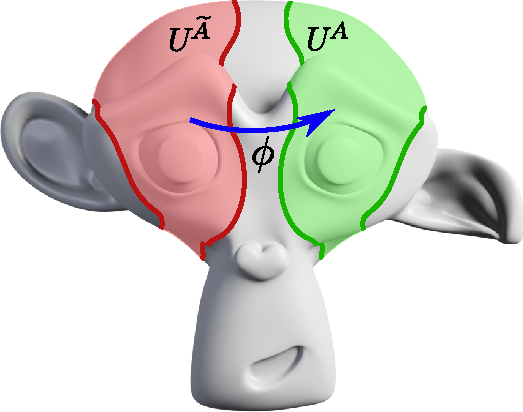
\includegraphics[width=.42\textwidth]{figures/suzanne_local_isometry.pdf}
    \hspace{2.ex}
    \captionsetup{width=.89\textwidth}
    \caption[]{\small
        یک منیفلد نامتقارن، که گروه ایزومتری \emph{سراسری} آن بدیهی است.
        از آنجایی که عدم تقارن به گوش‌ها و دهان
        «\href{https://en.wikipedia.org/wiki/Blender_(software)\#Suzanne}{سوزان}»،
        میمون، محدود می‌شود، تقارن‌های موضعی غیربدیهی باقی مانده‌اند.
        به عنوان مثال، نگاشت هموار ${\phi: U^{\widetilde{A}} \to U^A}$ بین زیرمجموعه‌های برجسته شده با رنگ قرمز و سبز، متریک را به صورت محلی حفظ می‌کند.
        تمام مفاهیم توسعه یافته در بخش~\ref{sec:isom_background} و همچنین هم‌متغیری ایزومتری عملیات نقطه‌ای مانند \onexones بلافاصله به چنین ایزومتری‌هایی بین زیرمجموعه‌های محلی تعمیم می‌یابد. 
        هم‌متغیری ایزومتری تبدیلات میدان کرنل با کرنل‌های با گستره فضایی تا اثرات مرزی تعمیم می‌یابد.
        }
    \label{fig:suzanne_local_isometry}
\end{SCfigure}











\subsubsection{عمل ایزومتری بر روی کلاف‌های تاری}
\label{sec:isom_action_bundles}

ایزومتری‌ها به طور طبیعی بر روی بردارهای مماس در $\TM$ و قاب‌های مرجع در $\FM$ با «حمل کردن آنها» با عمل گروهی همانطور که در شکل~\ref{fig:isom_egg_actions} به تصویر کشیده شده است، عمل می‌کنند.
اگر یک ایزومتری علاوه بر این با \lr{G}-ساختار سازگار باشد، یعنی اگر یک خودریختی از $\GM$ ایجاد کند، علاوه بر این بر روی هر کلاف \lr{G}-الحاقی، به ویژه کلاف‌های بردار ویژگی $\A$ عمل می‌کند.
ما این اعمال ایزومتری‌ها را بر روی کلاف‌های الحاقی و بر روی میدان‌های ویژگی در ادامه مورد بحث قرار می‌دهیم.



\paragraph{عمل ایزومتری بر روی کلاف مماس \lr{\textit{TM}}:}

هر ایزومتری $\phi \in \IsomM$ یک \emph{پیش‌ران} را ایجاد می‌کند
\begin{align}
    \dphiTM: \TM \to \TM \,, \qquad \phi\in \IsomM
\end{align}
روی کلاف مماس، که فقط دیفرانسیل $\phi$ است همانطور که در پیوست~\ref{apx:differentials_gradients_jacobians} معرفی شده است.
در هر نقطه $p \in M$ می‌توان آن را به عنوان یک تقریب \emph{خطی} از $\phi$ در نظر گرفت که بردارها $v \in \TpM$ را به $\dphiTM(v) \in T_{\mkern-1mu\phi(p)}\mkern-2mu M$ نگاشت می‌کند، یعنی برآورده می‌کند:
\begin{align}\label{eq:pushfwd_bundle_automorphism}
    \piTM \circ \dphiTM \,=\, \phi \circ \piTM.
\end{align}
همانطور که در پیوست~\ref{apx:differentials_gradients_jacobians} استدلال شد، پیش‌ران با $(\dphiTM)^{-1} = (\phi^{-1})_{\mkern-2mu*\mkern-1mu\scalebox{.55}{$,\mkern-2muT\mkern-3muM$}}$ معکوس‌پذیر است، که ما به طور بدون ابهام آن را با $\dphiTMinv$ خواهیم نوشت.%
\footnote{
    معکوس‌پذیری به طور کلی برای پیش‌ران‌ها برقرار نیست بلکه فقط برای پیش‌ران‌های دیفئومورفیسم‌ها و در نتیجه ایزومتری‌ها برقرار است.
}
بنابراین دیده می‌شود که پیش‌ران یک عنصر $\phi$ از گروه ایزومتری یک خودریختی کلاف برداری (ایزومتریک) از $\TM$ روی $\phi$ است که نمودار جابجایی زیر را برآورده می‌کند:
\begin{equation}\label{cd:pushforward_TM}
\begin{tikzcd}[column sep=70pt, row sep=40, font=\normalsize]
    \TM
        \arrow[r, shift left=2.5pt, "\dphiTM"]
        \arrow[d, "\piTM"']
    &
    \TM
        \arrow[d, "\piTM"]
        \arrow[l, shift left=2.5pt, "\dphiTMinv"]
    \\
    M
        \arrow[r, shift left=2.5pt, "\phi"]
    &
    M
        \arrow[l, shift left=2.5pt, "\phiinv"]
\end{tikzcd}
\end{equation}
بنا به \emph{تعریف ایزومتری‌ها}، پیش‌ران آنها فاصله‌ها و زوایا را حفظ می‌کند، یعنی،
\begin{align}\label{eq:metric_pushfwd_isometry}
    \eta_{\phi(p)} \big(\dphiTM v,\, \dphiTM w\big) \,=\, \eta_p(v,w)
    \qquad\ \forall\ \ p\in M,\ \  v,w\in \TpM,\ \ \phi \in \IsomM .
\end{align}
جزئیات بیشتر در مورد پیش‌ران‌ها بین کلاف‌های مماس به راحتی در ادبیات، به عنوان مثال در~\cite{schullerGeometricalAnatomy2016}، یافت می‌شود.



\paragraph{عمل ایزومتری بر روی کلاف قاب \lr{\textit{FM}}:}
پیش‌ران روی $\TM$ بلافاصله یک خودریختی کلاف اصلی متناظر $\dphiFM$ را بر روی $\FM$ با پیش‌ران کردن بردارهای قاب منفرد القا می‌کند:
\begin{align}\label{eq:pushforward_FM_def}
    \dphiFM\!: \FM \to \FM,\ \ \ 
    [e_i]_{i=1}^d \mapsto \dphiFM\big([e_i]_{i=1}^d\big) := \big[\dphiTM(e_i)\big]_{i=1}^d \,,
    \qquad \phi\in \IsomM
\end{align}
این نگاشت قاب‌ها را در $\FpM$ برای هر $p\in M$ دلخواه به قاب‌ها در $F_{\mkern-1mu\phi(p)}\mkern-2mu M$ نگاشت می‌کند، یعنی $\piFM \circ \dphiFM = \phi \circ \piFM$.
برای دیدن این، فرض کنید $[e_p]_{i=1}^d \in \FpM$، آنگاه $\phi\circ \piFM\big([e_i]_{i=1}^d\big) = \phi(p)$ و
$ \piFM \circ \dphiFM \big([e_i]_{i=1}^d\big)
= \piFM \pig(\big[ \dphiTM(e_i) \big]_{i=1}^d \pig)
= \piTM \circ \dphiTM (e_j)
= \phi \circ \piTM(e_j)
= \phi(p)$
برای هر $j=1,\dots,d$.
علاوه بر این می‌توان بررسی کرد که با
$(\dphiFM)^{-1} = (\phi^{-1})_{\mkern-2mu*\mkern-1mu\scalebox{.55}{$,\mkern-2mu F\mkern-3muM$}}$
معکوس‌پذیر است، که باز هم با $\dphiFMinv$ به اختصار نوشته می‌شود.
\emph{عمل چپ} $\dphiFM$ بر روی کلاف قاب با \emph{عمل راست} $\lhd$ بر روی تارهای آن جابجا می‌شود، یعنی برای هر $g\in \GL{d}$ و $\phi \in \IsomM$ دلخواه داریم:
\begin{alignat}{3}
\label{eq:dpsiFM_right_GL_equiv}
    \qquad
    \Big(\dphiFM \pig( [e_i]_{i=1}^d \pig)\Big) \lhd g
    \ &=\ \big[\dphiTM (e_i)\big]_{i=1}^d \lhd g
        \qquad\quad && \big( \text{\small تعریف $\dphiFM$، معادلۀ~\eqref{eq:pushforward_FM_def}} \big) \notag \\
    \ &=\ \Big[\sum\nolimits_j \dphiTM (e_j)\, g_{ji} \Big]_{i=1}^d
        \qquad\quad && \big( \text{\small تعریف $\lhd$، معادلۀ~\eqref{eq:rightaction_FM} } \big) \notag \\
    \ &=\ \Big[\dphiTM \Big(\sum\nolimits_je_j g_{ji}\Big) \Big]_{i=1}^d
        \qquad\quad && \big( \text{\small خطی بودن $\dphiTM$ } \big) \notag \\
    \ &=\ \dphiFM \Big(\Big[\sum\nolimits_je_j g_{ji}\Big] \Big)_{i=1}^d
        \qquad\quad && \big( \text{\small تعریف $\dphiFM$، معادلۀ~\eqref{eq:pushforward_FM_def}} \big) \notag \\
    \ &=\ \dphiFM \Big( [e_i]_{i=1}^d \lhd g \Big)
        \qquad\quad && \big( \text{\small تعریف $\lhd$، معادلۀ~\eqref{eq:rightaction_FM} } \big)
\end{alignat}
یک تبدیل پیمانه یک قاب در $p\in M$ با $g\in \GL{d}$، و به دنبال آن یک پیش‌ران به $\phi(p)$، بنابراین برابر است با یک پیش‌ران قاب تبدیل‌نشده، و به دنبال آن یک تبدیل پیمانه با همان عنصر گروهی $g$ اما در $\phi(p)$.
از این رو قاب‌های مختلف در تار $\FpM$ به گونه‌ای به قاب‌ها در $F_{\mkern-1mu\phi(p)}\mkern-2mu M$ نگاشت می‌شوند که جابجایی نسبی آنها حفظ شود.
ویژگی‌های استخراج شده از $\dphiFM$ با این گزاره خلاصه می‌شود که نمودار
\begin{equation}\label{eq:FM_isom_induced_automorphism}
\begin{tikzcd}[column sep=70pt, row sep=35, font=\normalsize]
    \FM
        \arrow[r, "\dphiFM"]
    &
    \FM
    \\
    \FM
        \arrow[r, "\dphiFM"]
        \arrow[d, "\piFM"']
        \arrow[u, "\lhd g"]
    &
    \FM
        \arrow[d, "\piFM"]
        \arrow[u, "\lhd g"']
    \\
    M
        \arrow[r, "\phi"']
    &
    M
\end{tikzcd}
\end{equation}
برای هر $\phi\in\IsomM$ و هر $g\in \GL{d}$ جابجا می‌شود.
با برآورده کردن جابجایی این نمودار، پیش‌ران $\dphiFM$ بر روی کلاف قاب به عنوان یک \emph{خودریختی کلاف اصلی} شناسایی می‌شود%
\footnote{
    یعنی، یک ایزومورفیسم کلاف اصلی از کلاف قاب به خودش؛ مقایسه کنید با معادله~\ref{cd:principal_bundle_morphism}.
}
روی $\phi$.

توجه داشته باشید که معکوس‌ها، که به طور صریح در نمودار~\eqref{cd:pushforward_TM} نشان داده شده‌اند، برای کاهش شلوغی حذف شده‌اند.






\paragraph{عمل ایزومتری بر روی \lr{G}-ساختارها \lr{\textit{GM}}:}

از آنجایی که \lr{G}-ساختارها زیرکلاف‌های اصلی از کلاف قاب هستند، می‌توان محدودیت دامنه پیش‌ران روی $\FM$ را به $\GM$ در نظر گرفت، یعنی،
\begin{align}
    \dphiFM \mkern-2mu \big|_{\scalebox{.58}{$\GM$}} :\ \GM \to \FM \,, \qquad \phi\in \IsomM \,.
\end{align}
در اینجا لازم است که کل کلاف قاب $\FM$ به عنوان هم‌دامنه حفظ شود زیرا به طور کلی هیچ تضمینی وجود ندارد که قاب‌ها در $\GpM$ به قاب‌های $\GphipM$ نگاشت شوند بلکه فقط به $\FphipM$ نگاشت می‌شوند.
\begin{figure}
    \centering
    \subcaptionbox{$\{e\}$-ساختار کانونی $\R^2$
        \label{fig:frame_field_automorphism_1}}%
        [.49\linewidth][l]{
            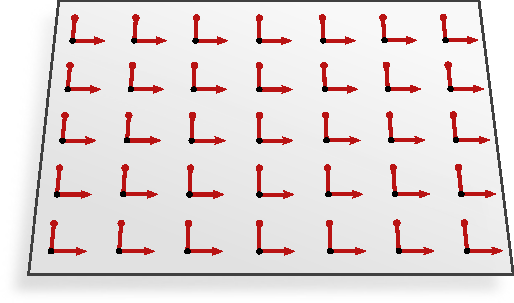
\includegraphics[width=.46\textwidth]{figures/frame_field_isom_equiv_1.pdf}
        }
    \subcaptionbox{یک $\{e\}$-ساختار جایگزین بر روی $\R^2$
        \label{fig:frame_field_automorphism_2}}%
        [.49\linewidth][l]{
            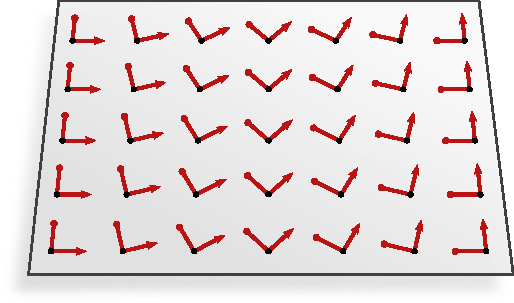
\includegraphics[width=.46\textwidth]{figures/frame_field_isom_equiv_2.pdf}
        }
    \caption[]{\small
        دو انتخاب خاص از $\{e\}$-ساختارها (میدان‌های قاب سراسری) $\eM$ روی $M = \R^2$ که ما برای به تصویر کشیدن مفهوم \emph{ایزومتری‌های حافظ \lr{G}-ساختار} از آنها استفاده می‌کنیم.
        گروه کامل ایزومتری $M$ گروه اقلیدسی $\IsomM=\E2$ است که از انتقال‌ها، دوران‌ها و بازتاب‌ها تشکیل شده است.
        شکل~\ref{fig:frame_field_automorphism_1} $\{e\}$-ساختار کانونی $\R^2$ را نشان می‌دهد که تحت انتقال‌ها نامتغیر است اما تحت دوران‌ها یا بازتاب‌ها نامتغیر نیست.
        به بیان انتزاعی‌تر، انتقال‌ها زیرگروه $\IsomeM = \Trans_2 := (\R^2,+)$ از ایزومتری‌هایی را تشکیل می‌دهند که خودریختی‌های $\eM$ را القا می‌کنند.
        در مقابل، دوران‌ها یا بازتاب‌ها قاب‌ها را در $\epM$ به قاب‌ها در $\FphipM$ نگاشت می‌کنند اما موفق به فرستادن آنها به $\ephipM$ نمی‌شوند.
        بنابراین آنها خودریختی‌های $\{e\}$-ساختار را القا نمی‌کنند و بخشی از $\IsomeM$ نیستند.
        اعمال گروهی چنین ایزومتری‌هایی بر روی $\eM$ یا هر یک از کلاف‌های $\{e\}$-الحاقی آن \emph{تعریف نشده است}.
        شکل~\ref{fig:frame_field_automorphism_2} یک انتخاب جایگزین از $\{e\}$-ساختار را بر روی $M = \R^2$ (یا $M=\Euc_2$) نشان می‌دهد که فقط تحت انتقال‌ها در جهت «بالا-پایین» نامتغیر است، یعنی $\IsomeM \cong \Trans_1 = (\R,+)$.
        مثال‌های موجود در شکل‌های~\ref{fig:frame_field_automorphism_1} و~\ref{fig:frame_field_automorphism_2} نمونه‌ای از این هستند که خودریختی‌های \lr{G}-ساختار نه تنها به گروه ساختار $G$ بلکه به انتخاب خاص \lr{G}-ساختار $\GM$ بستگی دارند.
        مورد کلی برای $G$ غیربدیهی سخت‌تر به تصویر کشیده می‌شود زیرا $\GpM$ در آن صورت یک قاب منفرد نخواهد بود بلکه مجموعه‌ای از قاب‌ها خواهد بود.
        }
    \label{fig:frame_field_automorphism}
\end{figure}
از آنجایی که \lr{G}-ساختارها به طور کلی تحت عمل ایزومتری‌ها بر روی $\FM$ بسته نیستند، ممکن است تعریف یک عمل گروهی از گروه کامل ایزومتری بر روی $\GM$ یا هر کلاف \lr{G}-الحاقی دیگر \emph{غیرممکن} باشد.
برای رفع این نقیصه، ما در ادامه زیرگروهی از آن ایزومتری‌ها را در نظر خواهیم گرفت که به \lr{G}-ساختار احترام می‌گذارند، یعنی قاب‌های ممتاز در $\GM$ را به قاب‌ها در $\GM$ نگاشت می‌کنند.
\begin{dfn}[ایزومتری‌های حافظ \lr{G}-ساختار]
\label{dfn:IsomGM}
    با داشتن یک \lr{G}-ساختار $\GM$، ما زیرگروه متناظر از ایزومتری‌های حافظ \lr{G}-ساختار $\IsomGM$ را به صورت زیر تعریف می‌کنیم:
    \begin{align}\label{eq:isomGM_def}
        \IsomGM\ :=\ \big\{ \phi \in \IsomM \,\big|\, \dphiFM(\GpM) = \GphipM\ \ \ \forall p \in M \big\} \ \leq\ \IsomM
    \end{align}
\end{dfn}
برای چنین ایزومتری‌هایی، ما عمل القایی بر روی $\GM$ را به صورت زیر تعریف می‌کنیم:
\begin{align}
    \dphiGM\, :=\, \dphiFM \mkern-2mu \big|_{\scalebox{.58}{$\GM$}} \,:\ \GM \to \GM \,, \qquad \phi\in \IsomGM \,.
\end{align}
اعمال تعریف‌شده به این شکل برای $\phi \in \IsomGM$ \emph{خودریختی‌های \lr{G}-ساختار} هستند، یعنی باعث می‌شوند نمودار زیر برای هر $g\in G$ جابجا شود (که با محدود کردن معادله~\eqref{eq:FM_isom_induced_automorphism} از $\FM$ به $\GM$ و از $\GL{d}$ به $G$ به دست می‌آید):
\begin{equation}\label{cd:isom_induced_GM_automorphism}
\begin{tikzcd}[column sep=70pt, row sep=35, font=\normalsize]
    \GM
        \arrow[r, "\dphiGM"]
    &
    \GM
    \\
    \GM
        \arrow[r, "\dphiGM"]
        \arrow[d, "\piGM"']
        \arrow[u, "\lhd g"]
    &
    \GM
        \arrow[d, "\piGM"]
        \arrow[u, "\lhd g"']
    \\
    M
        \arrow[r, "\phi"']
    &
    M
\end{tikzcd}
\end{equation}
شکل~\ref{fig:frame_field_automorphism} دو نمونه از $\{e\}$-ساختارها را روی $M=\R^2$ نشان می‌دهد، یعنی میدان‌های قاب سراسری.
از این مثال‌ها مشخص است که زیرگروه‌های $\IsomGM$ واقعاً به انتخاب خاص \lr{G}-ساختار $\GM$ بستگی دارند، نه فقط به گروه ساختار $G$.
در شکل~\ref{fig:SO2_structure_SE2} ما یک $\SO2$-ساختار را روی $M=\R^2$ به تصویر می‌کشیم.
گروه ایزومتری آن $\IsomSOM = \SE2$ بزرگتر از گروه‌های $\{e\}$-ساختارها در شکل~\ref{fig:frame_field_automorphism} است.
یک $\SO2$-ساختار روی کره $S^2$ که توسط تمام دوران‌ها $\IsomSOM = \SO3$ حفظ می‌شود، در شکل~\ref{fig:SO2_structure_SE2} نشان داده شده است.


برای انتخاب‌های خاص از گروه‌های ساختار $G$ می‌توان گزاره‌های کلی‌تری در مورد اینکه کدام ایزومتری‌ها در زیرگروه $\IsomGM$ قرار دارند، بیان کرد.
مهم‌تر از همه، برای گروه‌های ساختار اورتونرمال $G=\O{d}$ (که با $\eta$ سازگار هستند) \emph{هر} ایزومتری یک خودریختی از $\OM$ را القا می‌کند، یعنی همیشه داریم $\IsomOM = \IsomM \,.$
برای اثبات این ادعا، فرض کنید $[e_i]_{i=1}^d \in \OpM \subset \FpM$ یک قاب اورتونرمال باشد که توسط یک ایزومتری دلخواه $\phi \in \IsomM$ به $\dphiFM \big|_{\scalebox{.58}{$\OM$}} [e_i]_{i=1}^d = \big[\dphiTM e_i\big]_{i=1}^d$ فرستاده می‌شود؛ به معادله~\eqref{eq:pushforward_FM_def} مراجعه کنید.
اعمال معادله~\eqref{eq:metric_pushfwd_isometry} بر روی محورهای منفرد قاب پیش‌ران به دست می‌دهد:
\begin{align}\label{eq:isom_orthonormal_to_orthonormal_frames}
    \eta\big( \dphiTM e_i, \dphiTM e_j \big) \,=\, \eta(e_i, e_j) \,=\, \delta_{ij}\ \quad\ \forall\ \ i,j \in 1,\dots,d \,,
\end{align}
که اورتونرمال بودن قاب پیش‌ران $\dphiFM \big|_{\scalebox{.58}{$\OM$}} [e_i]_{i=1}^d \in \OphipM$ را ایجاب می‌کند و بنابراین اجازه می‌دهد تا $\dphiOM := \dphiFM \big|_{\scalebox{.58}{$\OM$}}$ را برای هر $\phi \in \IsomM$ تعریف کنیم.
به طور کلی‌تر، این نتیجه ایجاب می‌کند:
\begin{align}\label{eq:isomM_isomOM}
    \IsomGM = \IsomM \quad \ \forall\ G \geq \O{d}
\end{align}
به طور مشابه می‌توان نشان داد:
\begin{align}\label{eq:isomplusM_isomSOM}
    \IsomSOM = \IsomplusM \,,
\end{align}
یعنی، هر ایزومتری حافظ جهت در $\IsomplusM$ یک خودریختی از یک $\SO{d}$-ساختار $\SOM$ را القا می‌کند.
توجه داشته باشید که این گزاره‌ها همه فقط به گروه ساختار $G$ بستگی دارند اما از انتخاب خاص \lr{G}-ساختار مستقل هستند.
این در نهایت نتیجه در نظر گرفتن فقط ایزومتری‌ها است که بنا به تعریف با $\O{d}$-ساختارها سازگار هستند، به جای در نظر گرفتن دیفئومورفیسم‌های عمومی‌تر.
همانطور که قبلاً ذکر شد، زیرگروه $\IsomGM$ به طور کلی به انتخاب خاص \lr{G}-ساختار $\GM$ بستگی دارد، نه فقط به گروه ساختار $G$.


\begin{figure}
    \centering
    \subcaptionbox{$\SE2$-ساختار $\SO2$ نامتغیر $\SOM$ روی $M = \R^2$.
        \label{fig:SO2_structure_SE2}}%
        [.5\linewidth][l]{
            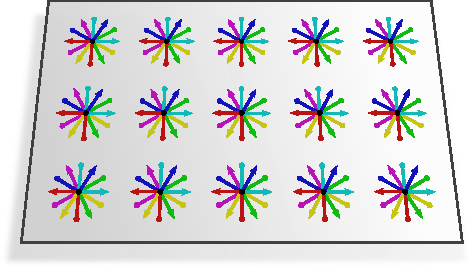
\includegraphics[width=.5\textwidth]{figures/SO2_structure_SE2.pdf}
            \rule{0pt}{20pt}
        }
    \subcaptionbox{$\SO3$-ساختار $\SO2$ نامتغیر $\SOM$ روی $M = S^2$\!\!.
        \label{fig:SO2_structure_SO3}}%
        [.48\linewidth][l]{
            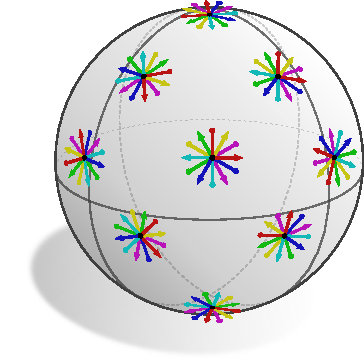
\includegraphics[width=.4\textwidth]{figures/SO2_structure_SO3.pdf}
        }
    \caption[]{\small
        دو نمونه از $\SO2$-ساختارها $\SOM$ روی صفحه $M = \R^2$ و کره $M = S^2$.
        برای ${M = \R^2}$، که در شکل~\ref{fig:SO2_structure_SE2} نشان داده شده است، $\SO2$-ساختار تحت انتقال‌ها و دوران‌ها نامتغیر است.
        از آنجایی که فقط از قاب‌های راست‌گرد تشکیل شده است (به نوک پیکان‌ها روی محورهای اول و نوک دایره‌ها روی محورهای دوم توجه کنید) تحت بازتاب‌ها نامتغیر نیست.
        بنابراین ایزومتری‌هایی که $\SOM$ را حفظ می‌کنند گروه $\IsomSOM = \SE2$ را تشکیل می‌دهند که زیرگروهی از گروه کامل ایزومتری $\IsomM = \E2$ است.
        در مورد $M = S^2$ که در شکل~\ref{fig:SO2_structure_SO3} نشان داده شده است، $\SO2$-ساختار تحت دوران‌ها نامتغیر است اما تحت بازتاب‌ها نامتغیر نیست.
        خودریختی‌های $\SO2$-ساختار در اینجا $\IsomSOM = \SO3$ هستند در حالی که گروه کامل ایzومتری $\IsomM = \O3$ است.
        }
    \label{fig:SO2_structures_SE2_SO3}
\end{figure}















\paragraph{عمل ایزومتری بر روی کلاف‌های برداری الحاقی $\A$:}
از پیش‌ران ایزومتری‌ها در $\IsomGM$ بر روی $\GM$ می‌توان یک پیش‌ران $\dphiA$ را بر روی هر کلاف برداری \lr{G}-الحاقی $\A = (\GM\times\R^c)/\!\sim_{\!\rho}$ با تعریف زیر ساخت:
\begin{align}\label{eq:pushforward_A_def}
    \dphiA\!: \A \to \A,\ \ \
    \pig[[e_i]_{i=1}^d,\, \mathscr{f}\pig]
    \mapsto \dphiA\!\Big(\! \pig[[e_i]_{i=1}^d,\, \mathscr{f}\pig] \!\Big)
    := \Big[\dphiGM \big([e_i]_{i=1}^d \big),\, \mathscr{f}\Big] \,,
    \qquad \phi \in \IsomGM \,.
\end{align}
این عمل خوش‌تعریف است زیرا ساختار به دلیل هم‌متغیری راست-\lr{G} $\dphiGM$ در معادله~\eqref{cd:isom_induced_GM_automorphism} از نماینده انتخاب‌شده کلاس هم‌ارزی مستقل است.
مشابه قبل، داریم $\piA\mkern2mu\circ\mkern2mu \dphiA = \phi\mkern2mu \circ\mkern2mu \piA$، یعنی $\dphiA$ بردارهای ویژگی را در $\A_p$ به بردارهای ویژگی در $\A_{\phi(p)}$ نگاشت می‌کند، که می‌توان با عمل بر روی یک بردار ویژگی و استفاده از ویژگی متناظر $\dphiGM$ آن را بررسی کرد.
از آنجایی که $\dphiA$ با عمل $\dphiGM$ بر روی عامل اول در $(\GM\times\R^c)/\!\sim_{\!\rho}$ تعریف می‌شود، با ترکیب‌های خطی که بر روی عامل دوم همانطور که در معادله~\eqref{eq:associated_bdl_linear_combination} تعریف شده است، عمل می‌کنند، تداخلی ندارد.
این ایجاب می‌کند که پیش‌ران روی کلاف‌های الحاقی به صورت خطی بین تارهای آنها نگاشت کند.
معکوس‌پذیری $\dphiA$ از معکوس‌پذیری $\dphiGM$ نتیجه می‌شود به طوری که دوباره داریم $(\dphiA)^{-1} = (\phi^{-1})_{\mkern-2mu*\mkern-1mu\scalebox{.55}{$,\mkern-2mu \A$}}$، که آن را به صورت $\dphiAinv$ می‌نویسیم.
این ویژگی‌ها، همراه با این واقعیت که $\dphiGM \in \Aut(\GM)$ به طور خاص یک خودریختی کلاف اصلی است، $\dphiA$ را به عنوان یک \emph{خودریختی کلاف برداری الحاقی} شناسایی می‌کند که نمودار جابجایی زیر را برآورده می‌کند:
\begin{equation}\label{cd:associated_bdl_automorphism}
\begin{tikzcd}[column sep=70pt, row sep=35, font=\normalsize]
    \A
        \arrow[r, "\dphiA"]
        \arrow[d, "\piA"']
    &
    \A
        \arrow[d, "\piA"]
    \\
    M
        \arrow[r, "\phi"']
    &
    M
\end{tikzcd}
\end{equation}

کلاف الحاقی حاصل از انتخاب‌های خاص نمایش گروهی $\rho(g)=g$ و $\R^d$ به عنوان تار نمونه‌ای از طریق مورفیسم کلاف $\chi:(\GM\times\R^d)/\!\!\sim\; \to \TM$ از معادله~\eqref{eq:A_TM_isomorphism} با کلاف مماس $\TM$ (به عنوان یک \lr{G}-کلاف) ایزومورف است.
تعریف ما از پیش‌ران‌ها بر روی کلاف‌های \lr{G}-الحاقی با این شناسایی سازگار است زیرا $\chi\circ\dphiA = \dphiTM\circ\chi$.
برای دیدن این، فرض کنید $\big[[e_i]_{i=1}^d,\, \mathscr{v}\big] \in (\GM\times\R^d)/\!\!\sim\;$ عنصری از کلاف الحاقی ایزومورف باشد که به $\chi\big(\big[ [e_i]_{i=1}^d,\, \mathscr{v} \big]\big) = \sum_i e_i \mathscr{v}_i$ نگاشت می‌شود.
آنگاه داریم
${\chi \circ \dphiA \big( \big[[e_i]_{i=1}^d,\, \mathscr{v}\big] \big)}
 = \chi \big( \big[[\dphiTM(e_i)]_{i=1}^d,\, \mathscr{v}\big] \big)
 = \sum_i \dphiTM(e_i) \mathscr{v}_i
 = \dphiTM \big(\sum_i e_i \mathscr{v}_i \big)
 = \dphiTM \circ \chi\big(\big[ [e_i]_{i=1}^d,\, \mathscr{v} \big]\big) \,,
$
که سازگاری تعاریف را نشان می‌دهد.


به عنوان یک کلاف الحاقی، پیش‌ران $\dphiHom$ بر روی کلاف هومومورفیسم $\Hom(\Ain,\Aout) \cong {(\GM\times\R^{\cout\times\cin})/\!\sim_{\!\rhoHom}}$ نیز با معادله~\eqref{eq:pushforward_A_def} مشخص می‌شود.
با این حال، ما بعداً به عبارتی از $\dphiHom$ بر حسب پیش‌ران‌های $\dphiAin$ و $\dphiAout$ از $\Ain$ و $\Aout$ نیاز خواهیم داشت، که آن را به زودی در اینجا استخراج خواهیم کرد.
برای این منظور، فرض کنید $H\in \Hom(\Ain|_p,\Aout|_p)$ یک هومومورفیسم در $p$ و $f_p\in \Ainp$ یک بردار ویژگی در $p$ باشد.
آنگاه $H(f_p)$ بنا به تعریف یک بردار ویژگی در $\Aoutp$ است.
برای اینکه به طور سازگار تعریف شود، پیش‌ران بردار ویژگی ورودی $f_p$ که توسط پیش‌ران هومومورفیسم $H$ بر آن عمل می‌شود، باید با پیش‌ران بردار ویژگی خروجی $H(f_p)$ موافق باشد.
این ایجاب می‌کند:
\begin{align}
    \dphiAout \big[ H(f_p) \big]
    \ =\  \big[ \dphiAout H\, \dphiAin^{-1} \big] \big( \dphiAin f_p \big)
    \ =:\ \big[ \dphiHom H \big] \big( \dphiAin f_p \big) \,,
\end{align}
که در آن پیش‌ران روی کلاف هومومورفیسم را به صورت زیر تعریف کردیم:
\begin{align}\label{eq:pushforward_Hom_def}
    \dphiHom\!: \Hom(\Ain,\Aout) \to \Hom(\Ain,\Aout), \quad
    H \mapsto
    \dphiAout H\, \dphiAininv \,,
    \qquad\ \phi \in \IsomGM
\end{align}
توجه داشته باشید که ترکیب یک عنصر $H\in \Hom(\Ain,\Aout)$ با $\dphiAout$ از چپ و با $\dphiAininv$ از راست، سبک معادله~\eqref{eq:Hom_bdl_triv_ptwise} را منعکس می‌کند.





\paragraph{عمل ایزومتری بر روی میدان‌های ویژگی:}
اعمال ایزومتری‌ها در $\IsomGM$ بر روی کلاف‌های الحاقی، اعمالی را بر روی مقاطع آنها، به ویژه بر روی میدان‌های ویژگی، ایجاد می‌کنند.
این پیش‌ران مقاطع به صورت زیر تعریف می‌شود:
\begin{dfn}[پیش‌ران ایزومتری میدان ویژگی:]
\label{dfn:isometry_pushforward}
    فرض کنید $f\in \Gamma(\A)$ یک میدان ویژگی و $\phi\in \IsomGM$ یک ایزومتری حافظ \lr{G}-ساختار باشد.
    ایزومتری از طریق \emph{پیش‌ران} بر روی میدان ویژگی عمل می‌کند%
    \footnote{
        به شباهت این تعریف با تعریف \emph{نمایش القایی} توجه کنید، که عمل گروهی است که شبکه‌های \lr{CNN} هدایت‌پذیر طوری طراحی شده‌اند که نسبت به آن هم‌متغیر باشند~\cite{Cohen2017-STEER,3d_steerableCNNs,Weiler2019_E2CNN}.
    }
    \begin{align}\label{eq:pushforward_section_A}
        \rhd\!:\ \IsomGM \mkern-2mu\times\mkern2mu \Gamma(\A) \to \Gamma(\A), \quad
        (\phi,f) \mapsto \phi\rhd\!f \,:=\, \dphiA\! \circ f \circ \phiinv \,.
    \end{align}
    بر حسب یک نمودار جابجایی، این تعریف به صورت زیر به تصویر کشیده می‌شود:
    \begin{equation}\label{cd:pushforward_section_A}
    \qquad\qquad
    \begin{tikzcd}[column sep=70pt, row sep=35, font=\normalsize]
        \A
            \arrow[r, "\dphiA"]
        &
        \A
        \\
        M
            \arrow[r, "\phi"']
            \arrow[u, "f\ "]
        &
        M
            \arrow[u, "\ \phi\rhd\!f\ :=\: \dphiA \!\circ\mkern-2mu f \circ \phiinv"']
    \end{tikzcd}
    \end{equation}
\end{dfn}
به طور شهودی، این تعریف بیان می‌کند که مقطع پیش‌ران $\phi\rhd\!f$ که در $p\in M$ ارزیابی می‌شود، بردار ویژگی $f$ را از $\phi^{-1}(p)$ که از طریق $\dphiA$ به $p$ پیش‌ران شده است، برمی‌گرداند.
توجه داشته باشید که چنین پیش‌ران‌هایی در واقع مقاطع خوش‌تعریفی را به دست می‌دهند که برآورده می‌کنند:
\begin{align}
    \piA \circ (\phi\rhd \!f)
    \ &=\ \piA \circ \dphiA\! \circ f \circ \phiinv \notag \\
    \ &=\ \phi \circ \piA \circ f \circ \phiinv \notag \\
    \ &=\ \phi \circ \id_M \circ \phiinv \notag \\
    \ &=\ \id_M
\end{align}
همانطور که در معادله~\eqref{cd:section_proj_idM} لازم است.
شکل~\ref{fig:isom_egg_actions} عمل ایزومتری‌ها را بر روی میدان‌ها به تصویر می‌کشد.
عمل ایزومتری‌ها بر روی پول‌بک منتقل‌کننده $\Expspf$ از میدان‌های $f$ در بخش~\ref{sec:isom_expmap_transport} در زیر استخراج می‌شود.

















\subsubsection{عمل ایزومتری در مختصات محلی}
\label{sec:isom_coordinatization}

بیشتر استخراج‌ها در مورد هم‌متغیری ایزومتری تبدیلات میدان کرنل در بخش‌های~\ref{sec:isometry_equivariance} و~\ref{sec:quotient_kernel_fields} در یک محیط مستقل از مختصات نگه داشته خواهند شد.
با این حال، از آنجایی که کانولوشن‌های $\GM$ نسبت به یک انتخاب از \lr{G}-اطلس‌های کلاف‌های الحاقی تعریف می‌شوند، بررسی هم‌متغیری ایزومتری آنها مستلزم مطالعه عبارات مختصاتی پیش‌ران‌های ایزومتری $\dphiTM$، $\dphiFM$، $\dphiGM$ و $\dphiA$ نسبت به بدیهی‌سازی‌های محلی کلاف است.
عبارات مختصاتی عمل ایزومتری علاوه بر این در پیاده‌سازی‌های عددی مفید هستند، که لزوماً میدان‌های ویژگی را نسبت به میدان‌های قاب‌های مرجع کدگذاری می‌کنند.

در ادامه، ما پیمانه‌های $\PsiTM^{\widetilde{A}}$ و $\PsiTM^A$ را به ترتیب در همسایگی‌های $U^{\widetilde{A}}$ از $p$ و $U^A$ از $\phi(p)$ داده شده فرض می‌کنیم.
برای راحتی، فرض کنید $U^A = \phi\big(U^{\widetilde{A}}\big)$ با تصویر $U^{\widetilde{A}}$ تحت ایزومتری منطبق باشد، که همیشه بدون از دست دادن کلیت امکان‌پذیر است.




\paragraph{پیش‌ران روی \lr{\textit{TM}} در مختصات:}
به یاد بیاورید که پیش‌ران روی کلاف مماس یک نگاشت خطی از بردارها $v\in \TpM$ به بردارها $\dphiTM v \in \TphipM$ است.
نسبت به پیمانه‌های داده شده، پیش‌ران بنابراین توسط یک میدان از ماتریس‌ها مختصاتی می‌شود%
\footnote{
    با داشتن چارت‌های
    $x^{\widetilde{A}}: U^{\widetilde{A}} \to x^{\widetilde{A}}\big(U^{\widetilde{A}}\big) \subseteq \R^d$
    و
    $x^A: U^A \to x^A\big(U^A\big) \subseteq \R^d$
    از $M$، یک ایزومتری $\phi$ را می‌توان به صورت محلی با یک نگاشت
    $x^A \circ \phi \circ \big(x^{\widetilde{A}}\big)^{\mkern-1mu-1}\!: x^{\widetilde{A}}\big(U^{\widetilde{A}}\big) \to x^A\big(U^A\big)$
    بین مختصات نمایش داد.
    برای حالت خاصی که پیمانه‌ها در $p$ و $\phi(p)$ متناظر با پایه‌های مختصاتی آن چارت‌ها هستند، $g_\phi^{A\widetilde{A}}$ به سادگی توسط \emph{ژاکوبین} $x^A \circ \phi \circ \big(x^{\widetilde{A}}\big)^{\mkern-1mu-1}$ داده می‌شود.
}
\begin{align}\label{eq:pushforward_TM_coord}
    g_\phi^{A\widetilde{A}}\!: U^{\widetilde{A}} \to \GL{d},\ \ \ 
    p \mapsto g_\phi^{A\widetilde{A}}(p) := \psiTMphip^A \mkern-2mu\circ \dphiTM \mkern-2mu\circ \big(\psiTMp^{\widetilde{A}}\big)^{-1}
    , \quad\ \ \phi \in \IsomM \,,
\end{align}
که بین ضرایب عددی متناظر $\psiTMp^{\widetilde{A}}(v)$ از $v$ در $p$ و $\psiTMphip^A(\dphiTM v) = g_\phi^{A\widetilde{A}}(p) \psiTMp^{\widetilde{A}}(v)$ از $\dphiTM v$ در $\phi(p)$ تبدیل می‌کند.
دقیق‌تر، $g_\phi^{A\widetilde{A}}$ در زیرگروه $\langle\, G\cup\O{d} \,\rangle$ از $\GL{d}$ مقدار می‌گیرد، که توسط عناصر $\O{d}$ (به دلیل اینکه $\dphiTM$ متریک را حفظ می‌کند) و $G$ (زیرا توابع گذار ممکن است یک ابرگروه از $\O{d}$ تشکیل دهند) تولید می‌شود.
تعریف پیش‌ران در مختصات محلی با نمودار جابجایی زیر به تصویر کشیده می‌شود:
\begin{equation}\label{cd:pushforward_TM_coord}
    \begin{tikzcd}[row sep=4.em, column sep=5em]
        \R^d
            \arrow[rrr, pos=.5, rounded corners, to path={ 
                    -- ([yshift=-3.5ex]\tikztostart.south) 
                    --node[below]{\small$
                        g_\phi^{A\widetilde{A}}(p) \mkern2mu\cdot
                        $} ([yshift=-3.5ex]\tikztotarget.south) 
                    -- (\tikztotarget.south)
                    }]
        &
        \TpM
            \arrow[l, "\psiTMp^{\widetilde{A}}"']
            \arrow[r, "\dphiTM"]
        &
        \TphipM
            \arrow[r, "\psiTMphip^A"]
        &
        \R^d
    \end{tikzcd}
\end{equation}
شکل~\ref{fig:pushforward_vector_components} یک تفسیر گرافیکی از پیش‌ران در مختصات ارائه می‌دهد.


\paragraph{پیش‌ران روی \lr{\textit{FM}} در مختصات:}
مختصاتی‌سازی پیش‌ران روی کلاف قاب به قیاس با معادله~\eqref{eq:pushforward_TM_coord} تعریف می‌شود.
مشخص می‌شود که این با عمل چپ همان عنصر گروهی $g_\phi^{A\widetilde{A}}$ بر روی قاب‌های بدیهی‌شده داده می‌شود همانطور که در نمودار جابجایی زیر نشان داده شده است:
\begin{equation}\label{eq:pushforward_FM_coord}
    \begin{tikzcd}[row sep=4.em, column sep=5em]
        \GL{d}
            \arrow[rrr, pos=.5, rounded corners, to path={ 
                    -- ([yshift=-3.5ex]\tikztostart.south) 
                    --node[below]{\small$
                        g_\phi^{A\widetilde{A}}(p) \mkern2mu\cdot
                        $} ([yshift=-3.5ex]\tikztotarget.south) 
                    -- (\tikztotarget.south)
                    }]
        &
        \FpM
            \arrow[l, "\psiFMp^{\widetilde{A}}"']
            \arrow[r, "\dphiFM"]
        &
        \FphipM
            \arrow[r, "\psiFMphip^A"]
        &
        \GL{d}
    \end{tikzcd}
\end{equation}
برای اثبات این ادعا، ما عمل را بر روی یک قاب بدیهی‌شده، که با یک ماتریس $h \in \GL{d}$ که ستون $i$-ام آن $h_{:,i}$ نماینده بردار قاب $i$-ام است، محاسبه می‌کنیم:
\begin{alignat}{3}
    \qquad\qquad
        & \Big[ \psiFMphip^A \circ \dphiFM \circ \big(\psiFMp^{\widetilde{A}}\big)^{-1} \Big](h) \notag \\
    =\ & \Big[ \psiFMphip^A \circ \dphiFM \Big] \!\Big( \!\Big( \big(\psiTMp^{\widetilde{A}}\big)^{-1} (h_{:,i})\Big)_{i=1}^d \Big)
        \qquad\quad && \big( \text{\small تعریف $\psiFMp^{\widetilde{A}}$، معادلۀ~\eqref{eq:trivialization_FM_p} } \big) \notag \\
    =\ & \psiFMphip^A \!\Big( \!\Big( \dphiTM \circ \big(\psiTMp^{\widetilde{A}}\big)^{-1} (h_{:,i})\Big)_{i=1}^d \Big)
        \qquad\quad && \big( \text{\small تعریف $\dphiFM$، معادلۀ~\eqref{eq:pushforward_FM_def} } \big) \notag \\
    =\ & \Big( \!\Big( \psiTMphip^A \circ \dphiTM \circ \big(\psiTMp^{\widetilde{A}}\big)^{-1} (h_{:,i})\Big)_{i=1}^d \Big)
        \qquad\quad && \big( \text{\small تعریف $\psiFMphip^A$، معادلۀ~\eqref{eq:trivialization_FM_p} } \big) \notag \\
    =\ & \Big( g_\phi^{A\widetilde{A}}(p) \cdot h_{:,i} \Big)_{i=1}^d
        \qquad\quad && \big( \text{\small تعریف $g_\phi^{A\widetilde{A}}$، معادلۀ~\eqref{eq:pushforward_TM_coord} } \big) \notag \\
    =\ & g_\phi^{A\widetilde{A}}(p) \cdot h
\end{alignat}


عمل پیش‌ران بر روی بدیهی‌سازی‌های محلی را می‌توان به عنوان \emph{القا کردن یک تبدیل پیمانه} در نظر گرفت.
یک شهود گرافیکی برای این گزاره در شکل~\ref{fig:pushforward_vector_components} داده شد که در آن پیمانه‌های اولیه در $p$ و $\phi(p)$ با انتخاب‌های قاب‌های مرجع به تصویر کشیده شده‌اند.
یک پیش‌ران از قاب در $p$ به $\phi(p)$ (قرمز) به طور کلی با قاب اصلی در $\phi(p)$ (سبز) موافق نیست.
گذار بین این دو قاب، تبدیل پیمانه القا شده در $\phi(p)$ است.
ما در ادامه این تبدیل را می‌سازیم؛ ابتدا بر حسب بدیهی‌سازی‌های محلی، سپس بر حسب میدان‌های قاب متناظر.


از نمودار جابجایی در معادله~\eqref{eq:pushforward_FM_coord} مشخص است که پیمانه $\psiFMp^{\widetilde{A}}: \FpM \to \GL{d}$ در $p$ را می‌توان از طریق $\dphiFM^{-1}$ به یک پیمانه در $\phi(p)$ پول‌بک کرد، که به صورت زیر داده می‌شود:
\begin{align}\label{eq:isom_pullback_section_FM}
    \psiFMp^{\widetilde{A}} \circ \dphiFM^{-1}
    \ =\ \big( g_\phi^{A\widetilde{A}}(p) \big)^{-1} \psiFMphip^A
    \,:\,\ \FphipM \to \GL{d} \,.
\end{align}
گسترش متناظر نمودار جابجایی در معادله~\eqref{eq:pushforward_FM_coord} هم‌ارزی هر دو عبارت را به تصویر می‌کشد و یک اثبات جبری را زائد می‌کند:
\begin{equation}\label{cd:pushforward_FM_coord_extended}
    \begin{tikzcd}[row sep=4.em, column sep=5em]
        \GL{d}
            \arrow[rrr, pos=.5, rounded corners, to path={ 
                    -- ([yshift=-3.5ex]\tikztostart.south) 
                    --node[below]{\small$
                        g_\phi^{A\widetilde{A}}(p) \mkern2mu\cdot
                        $} ([yshift=-3.5ex]\tikztotarget.south) 
                    -- (\tikztotarget.south)
                    }]
        &
        \FpM
            \arrow[l, "\psiFMp^{\widetilde{A}}"']
            \arrow[r, "\dphiFM"]
        &
        \FphipM
            \arrow[r, "\psiFMphip^A"]
            \arrow[ll, pos=.5, rounded corners, to path={ 
                    -- ([yshift=5.ex]\tikztostart.north) 
                    --node[above]{\small$
                        \psiFMp^{\widetilde{A}}\, \dphiFM^{-1}\ =\ 
                        \big( g_\phi^{A\widetilde{A}}(p) \big)^{-1} \mkern-2mu\cdot \psiFMphip^A
                        $} ([yshift=5.ex]\tikztotarget.north) 
                    -- (\tikztotarget.north)
                    }]
        &
        \GL{d}
    \end{tikzcd}
\end{equation}
نگاشت گذار (تبدیل پیمانه) بین پیمانه القا شده از ایزومتری $\psiFMp^{\widetilde{A}} \, \dphiFM^{-1}$ و پیمانه اصلی $\psiFMphip^A$ در $\phi(p)$ مشخص می‌شود که توسط عنصر گروهی معکوس داده می‌شود%
\footnote{
    معکوس یک موضوع قراردادی است.
    در اینجا به این دلیل به وجود می‌آید که ما $g_\phi^{A\widetilde{A}}$ را به عنوان عبارت مختصاتی پیش‌ران هموردای قاب‌ها تعریف کردیم در حالی که پیمانه‌ها به صورت پادوردا تبدیل می‌شوند.
}
\begin{align}\label{eq:gauge_trafo_pushforward_gauge}
    \big( \psiFMp^{\widetilde{A}} \, \dphiFM^{-1} \big) \circ \big( \psiFMphip^A \big)^{-1}
    \ =\ \big( g_\phi^{A\widetilde{A}}(p) \big)^{-1}
    \ \ \ \in\,\ \langle\, G\cup\O{d} \,\rangle\ \leq\ \GL{d} \,.
\end{align}
توجه داشته باشید که این عنصر گروهی برای $G\leq\O{d}$ لزوماً در گروه ساختار قرار نمی‌گیرد، یعنی پیمانه القا شده از ایزومتری ممکن است \lr{G}-سازگار نباشد (نمی‌توان آن را به یک \lr{G}-اطلس موجود از $\FM$ اضافه کرد).
در پاراگراف بعدی در مورد \lr{G}-ساختارها نشان خواهیم داد که این دقیقاً زمانی اتفاق می‌افتد که $\phi \notin \IsomGM$ باشد، یعنی برای ایزومتری‌هایی که به \lr{G}-ساختار احترام نمی‌گذارند.


برای استخراج عمل ایزومتری بر روی میدان‌های قاب، مقاطع همانی $\sigma^{\widetilde{A}}: U^{\widetilde{A}} \to \piFM^{-1}\big(U^{\widetilde{A}}\big)$ روی $U^{\widetilde{A}}$ و $\sigma^A: U^A \to \piFM^{-1}\big(U^A\big)$ روی $U^A$ را در نظر بگیرید.
این مقاطع میدان‌های قاب اصلی را از شکل~\ref{fig:pushforward_vector_components} مدل می‌کنند.
سپس میدان قاب جدید با مقطع پیش‌ران داده می‌شود:
\begin{align}\label{eq:pushforward_section_FM}
    \phi \mkern2mu\rhd \sigma^{\widetilde{A}} \,:=\, \dphiFM \circ \sigma^{\widetilde{A}} \circ \phiinv
    \ :\ U^A \to \piFM^{-1}\big( U^A\big) \,,
\end{align}
که به طور معادل با تعریف در معادله~\ref{eq:pushforward_section_A} تعریف شده است.
یک عبارت جایگزین برای میدان قاب پیش‌ران بر حسب عمل راست $g_\phi^{A\widetilde{A}}$ با اعمال $\psiFMphip^A$ یافت می‌شود:
\begin{alignat}{3}
    \qquad\qquad\qquad
        &\ \ \psiFMphip^A \pig(\big[ \phi \rhd \sigma^{\widetilde{A}} \,\big] (\phi(p)) \pig) \notag \\
    =&\ \ \psiFMphip^A \, \dphiFM \, \sigma^{\widetilde{A}}(p)
        \qquad\quad && \big( \text{\small تعریف $\phi \rhd \sigma^{\widetilde{A}}$، معادلۀ~\eqref{eq:pushforward_section_FM} } \big) \notag \\
    =&\ \ g_\phi^{A\widetilde{A}}(p) \, \psiFMp^{\widetilde{A}} \, \sigma^{\widetilde{A}}(p) 
        \qquad\quad && \big( \text{\small عبارات معادل در معادلۀ~\eqref{eq:isom_pullback_section_FM} } \big) \notag \\
    =&\ \ g_\phi^{A\widetilde{A}}(p)
        \qquad\quad && \big( \text{\small مقطع همانی $\sigma^{\widetilde{A}}$، معادلۀ~\eqref{eq:identity_section_prop} } \big) \notag \\
    =&\ \ \psiFMphip^A \pig( \sigma^A \big(\phi(p)\big) \pig) \, g_\phi^{A\widetilde{A}}(p)
        \qquad\quad && \big( \text{\small مقطع همانی $\sigma^A$، معادلۀ~\eqref{eq:identity_section_prop} } \big) \notag \\
    =&\ \ \psiFMphip^A \pig( \sigma^A \big(\phi(p)\big) \lhd g_\phi^{A\widetilde{A}}(p) \pig)
        \qquad\quad && \big( \text{\small هم‌متغیری راست-$\GL{d}$، معادلۀ~\eqref{eq:right_equivariance_FM} } \big)
\end{alignat}
از آنجایی که $\psiFMphip^A$ یک ایزومورفیسم است، نتیجه می‌شود که:
\begin{align}\label{eq:pushfwd_section_right_action}
    \pig(\phi \rhd \sigma^{\widetilde{A}} \pig) \big( \phi(p) \big)
    \ =\ \dphiFM \sigma^{\widetilde{A}} (p)
    \ =\ \sigma^A \big(\phi(p)\big) \lhd g_\phi^{A\widetilde{A}}(p) \,,
\end{align}
یعنی، $g_\phi^{A\widetilde{A}}(p)$ همانطور که انتظار می‌رفت تبدیل بین مقاطع همانی را توصیف می‌کند.
این تبدیل القا شده از ایزومتری بین قاب‌های مرجع در شکل~\ref{fig:pushforward_vector_components} با فلش آبی بین قاب قرمز (شفاف) و سبز به تصویر کشیده شده است.


پیمانه تبدیل‌شده با ایزومتری $\psiFMp^{\widetilde{A}}\, \dphiFM^{-1}$ و مقطع پیش‌ران $\phi \rhd \sigma^{\widetilde{A}}$ به این ترتیب با یکدیگر مطابقت دارند که دومی مقطع همانی اولی است:
\begin{align}
    \psiFMp^{\widetilde{A}}\, \dphiFM^{-1} \pig[ \phi \rhd \sigma^{\widetilde{A}} \pig] \big(\phi(p)\big)
    \ =\ \psiFMp^{\widetilde{A}}\, \dphiFM^{-1} \dphiFM \sigma^{\widetilde{A}}(p)
    \ =\ \psiFMp^{\widetilde{A}} \sigma^{\widetilde{A}}(p)
    \ =\ e
\end{align}






\paragraph{پیش‌ران روی \lr{\textit{GM}} در مختصات:}
همانطور که در بخش قبلی~\ref{sec:isom_action_bundles} استدلال شد، پیش‌ران روی $\GM$ فقط برای ایزومتری‌های $\phi$ در یک زیرگروه $\IsomGM$ خوش‌تعریف است.
جای تعجب نیست که تبدیلات پیمانه القا شده از ایزومتری متناظر در گروه ساختار $G$ مقدار می‌گیرند:
\begin{thm}[$\IsomGM$ در بدیهی‌سازی‌های محلی]
\label{thm:isom_GM_in_coords}
    فرض کنید $\phi \in \IsomM$ هر ایزومتری از $M$ باشد.
    آنگاه سه گزاره زیر معادل هستند:
    \begin{enumerate}
        \item $\phi$ حافظ \lr{G}-ساختار است، یعنی $\phi \in \IsomGM$.
        \item پول‌بک ایزومتری $\psiFMp^{\widetilde{A}}\, \dphiFM^{-1}$ از هر پیمانه $\psiFMp^{\widetilde{A}}$ از \lr{G}-اطلس $\FM$ که $\GM$ را تعریف می‌کند، با آن \lr{G}-اطلس \lr{G}-سازگار است.
        \item
        عبارت مختصاتی $\dphiFM$ نسبت به هر پیمانه $\psiFMp^{\widetilde{A}}$ و $\psiFMphip^A$ از \lr{G}-اطلس $\FM$ در گروه ساختار مقدار می‌گیرد، یعنی $g_\phi^{A\widetilde{A}}(p) \in G\ \ \ \forall\ p \in M$.
    \end{enumerate}
\end{thm}
\begin{proof}
    ویژگی تعریف‌کننده یک ایزومتری حافظ \lr{G}-ساختار $\phi \in \IsomGM$ این است که $\dphiFM(\GpM) = \GphipM$ را برای هر $p \in M$ برآورده می‌کند؛ به معادله~\eqref{eq:isomGM_def} مراجعه کنید.
    بر حسب یک \lr{G}-اطلس داده شده از $\FM$، معادله~\eqref{eq:G_atlas_induced_G_structure_GM_def_ptwise} \lr{G}-ساختار را در $p\in M$ به صورت $\GpM := \big(\psiFMp^{\widetilde{A}}\big)^{-1} (G)$ تعریف کرد که در آن $\psiFMp^{\widetilde{A}}$ یک پیمانه \emph{دلخواه} از \lr{G}-اطلس است.
    با این عبارت ما سمت چپ ویژگی تعریف‌کننده $\IsomGM$ را بسط می‌دهیم:
    \begin{align}
        \dphiFM(\GpM)
        \ &=\ \dphiFM\, \big(\psiFMp^{\widetilde{A}}\big)^{-1} (G) \notag \\
        \ &=\ \Big(\psiFMp^{\widetilde{A}} \dphiFM^{-1} \Big)^{-1} (G)
    \intertext{
    نسبت به هر پیمانه $\psiFMphip^A$ از \lr{G}-اطلس در $\phi(p)$، این را می‌توان بیشتر به صورت زیر دستکاری کرد
    }
        \dphiFM(\GpM)
        \ &=\ \Big(\big( g_\phi^{A\widetilde{A}}(p) \big)^{-1} \psiFMphip^A  \Big)^{-1} (G) \notag \\
        \ &=\ \big( \psiFMphip^A   \big)^{-1} \big(g_\phi^{A\widetilde{A}}(p)\, G\big) \,.
    \end{align}
    سمت راست ویژگی تعریف‌کننده $\IsomGM$ بر حسب $\psiFMphip^A$ به صورت زیر داده می‌شود:
    \begin{align}
        \GphipM = \big( \psiFMphip^A \big)^{-1} (G).
    \end{align}
    با برابر قرار دادن هر دو طرف و استفاده از اینکه $\psiFMphip^A$ یک ایزومورفیسم است، نتیجه می‌شود $g_\phi^{A\widetilde{A}}(p)\, G = G$ که به هم‌ارزی ادعا شده منجر می‌شود:
    \begin{align}
        \dphiFM(\GpM) = \GphipM
        \quad \Longleftrightarrow \quad
        g_\phi^{A\widetilde{A}}(p) \in G
    \end{align}
    از گزاره‌های \textit{1}. و \textit{3}.
    برای اثبات هم‌ارزی با گزاره~\textit{2.}، به یاد بیاورید که $g_\phi^{A\widetilde{A}}(p)$ طبق معادله~\eqref{eq:gauge_trafo_pushforward_gauge} برابر با تبدیل پیمانه از $\psiFMp^{\widetilde{A}} \, \dphiFM^{-1}$ به $\psiFMphip^A$ است.
    از آنجایی که \lr{G}-اطلس‌ها بنا به تعریف توابع گذار در گروه ساختار $G$ دارند، پیامدهای (\textit{2.$\leftrightarrow$3.}) نتیجه می‌شوند، به طوری که هر سه گزاره معادل دیده می‌شوند.
\end{proof}
این نتایج برای مطالعه بعدی ما در مورد هم‌متغیری ایزومتری کانولوشن‌های $\GM$ اهمیت مرکزی دارند.
ما قادر خواهیم بود نشان دهیم که چنین کانولوشن‌هایی تحت عمل $\phi \in \IsomGM$ بر روی میدان‌های ویژگی هم‌متغیر هستند، که به این واقعیت متکی است که \lr{G}-هدایت‌پذیری کرنل‌های کانولوشن، تبدیلات پیمانه القا شده از ایزومتری $g_\phi^{A\widetilde{A}}(p) \in G$ را در نظر می‌گیرد.


برای ایزومتری‌های القاکننده خودریختی \lr{G}-ساختار $\phi \in \IsomGM$، ما می‌توانیم نمودار جابجایی برای $\FM$ در معادله~\eqref{cd:pushforward_FM_coord_extended} را به همتای آن برای $\GM$ تطبیق دهیم:
\begin{equation}\label{cd:pushforward_GM_coord_extended}
    \begin{tikzcd}[row sep=4.em, column sep=5em]
        G
            \arrow[rrr, pos=.5, rounded corners, to path={ 
                    -- ([yshift=-3.5ex]\tikztostart.south) 
                    --node[below]{\small$
                        g_\phi^{A\widetilde{A}}(p) \mkern2mu\cdot
                        $} ([yshift=-3.5ex]\tikztotarget.south) 
                    -- (\tikztotarget.south)
                    }]
        &
        \GpM
            \arrow[l, "\psiGMp^{\widetilde{A}}"']
            \arrow[r, "\dphiGM"]
        &
        \GphipM
            \arrow[r, "\psiGMphip^A"]
            \arrow[ll, pos=.5, rounded corners, to path={ 
                    -- ([yshift=5.ex]\tikztostart.north) 
                    --node[above]{\small$
                        \psiGMp^{\widetilde{A}}\, \dphiGM^{-1}\ =\ 
                        \big( g_\phi^{A\widetilde{A}}(p) \big)^{-1} \mkern-2mu\cdot \psiGMphip^A
                        $} ([yshift=5.ex]\tikztotarget.north) 
                    -- (\tikztotarget.north)
                    }]
        &
        G
    \end{tikzcd}
\end{equation}
















\paragraph{پیش‌ران روی $\A$ در مختصات:}

پیش‌ران $\phi \in \IsomGM$ بر روی کلاف‌های \lr{G}-الحاقی به طور مشابه با پیش‌ران‌های دیگر کلاف‌ها مختصاتی می‌شود.
بر حسب یک نمودار جابجایی، ما به طور غیرمنتظره‌ای به دست می‌آوریم:
\begin{equation}\label{cd:pushforward_A_coord_persian}
    \quad
    \begin{tikzcd}[row sep=4.em, column sep=5em]
        \R^c
            \arrow[rrr, pos=.5, rounded corners, to path={ 
                    -- ([yshift=-3.5ex]\tikztostart.south) 
                    --node[below]{\small$
                        \rho\big( g_\phi^{A\widetilde{A}}(p) \big)
                        $} ([yshift=-3.5ex]\tikztotarget.south) 
                    -- (\tikztotarget.south)
                    }]
        &
        \A_p
            \arrow[l, "\psiAp^{\widetilde{A}}"']
            \arrow[r, "\dphiA"]
        &
        \A_{\phi(p)}
            \arrow[r, "\psiAphip^A"]
        &
        \R^c
    \end{tikzcd}
    \quad,
\end{equation}
که وقتی بر روی ضرایب بردار ویژگی $\mathscr{f}\in\R^c$ عمل می‌کنیم به دست می‌آید:
\begin{alignat}{3}
    \qquad\qquad\qquad\qquad\quad
        & \Big[ \psiAphip^A \circ \dphiA \circ \big(\psiAp^{\widetilde{A}}\big)^{-1} \Big] (\mathscr{f}) \notag \\
    =\ & \Big[ \psiAphip^A \circ \dphiA \Big] \!\Big( \Big[ \sigma^{\widetilde{A}}(p), \,\mathscr{f}\, \Big] \Big)
        \qquad\quad && \big( \text{\small تعریف $\big(\psiAp^A\big)^{-1}$، معادلۀ~\eqref{eq:trivialization_A_p_inv} } \big) \notag \\
    =\ & \psiAphip^A \!\Big( \Big[ \dphiFM\big( \sigma^{\widetilde{A}}(p) \big), \,\mathscr{f}\, \Big] \Big)
        \qquad\quad && \big( \text{\small تعریف $\dphiA$، معادلۀ~\eqref{eq:pushforward_A_def} } \big) \notag \\
    =\ & \psiAphip^A \!\Big( \Big[ \sigma^A\big(\phi(p)\big) \lhd g_\phi^{A\widetilde{A}}(p), \,\mathscr{f}\, \Big] \Big)
        \qquad\quad && \big( \text{\small تبدیل پیمانه القایی، معادلۀ~\eqref{eq:pushfwd_section_right_action} } \big) \notag \\
    =\ & \psiAphip^A \!\Big( \Big[ \sigma^A\big(\phi(p)\big), \, \rho\big( g_\phi^{A\widetilde{A}}(p) \big) \mathscr{f}\, \Big] \Big)
        \qquad\quad && \big( \text{\small تعریف $\sim_{\!\rho}$، معادلۀ~\eqref{eq:equiv_relation_A} } \big) \notag \\
    =\ & \rho\Big( g_\phi^{A\widetilde{A}}(p) \Big) \cdot \mathscr{f}
        \qquad\quad && \big( \text{\small تعریف $\psiAp$، معادلۀ~\eqref{eq:trivialization_A_p} } \big)
\end{alignat}
توجه داشته باشید که عبارت $\rho\big( g_\phi^{A\widetilde{A}}(p) \big)$ مستلزم آن است که $g_\phi^{A\widetilde{A}}(p)$ یک عنصر گروه ساختار باشد زیرا $\rho$ یک نمایش \lr{G} است.
این یک بار دیگر از دیدگاه دیگری نشان می‌دهد که پیش‌ران‌ها بر روی $\A$ فقط می‌توانند برای ایزومتری‌ها در $\IsomGM$ تعریف شوند.

برای کامل بودن، ما بدیهی‌سازی محلی زیر از نمودار جابجایی از معادله~\eqref{cd:pushforward_section_A} را ارائه می‌دهیم، که ممکن است هنگام پیاده‌سازی \lr{CNN}های مستقل از مختصات و آزمایش هم‌متغیری $\IsomGM$ آنها مفید باشد:
\begin{equation}\label{cd:pushforward_A_coord}
\begin{tikzcd}[column sep=60pt, row sep=45, font=\normalsize,
               execute at end picture={
                    \node [] at (-1.87, -.07) {$\noncommutative$};
                    \node [] at ( 1.87, -.07) {$\noncommutative$};
                    }]
    U^{\widetilde{A}} \times \R^c
        \arrow[rd, "\proj_1"']
        \arrow[rrr, rounded corners, to path={ 
                -- ([yshift=2em]\tikztostart.north) 
                --node[above]{\small$\phi \times \rho\big(g^{A\widetilde{A}}_\phi\big) \cdot$} ([yshift=2em]\tikztotarget.north) 
                -- (\tikztotarget.north)
                }]
    &
    \piA^{-1}\big(U^{\widetilde{A}}\big)
        \arrow[r, "\dphiA"]
        \arrow[d, "\piA"']
        \arrow[l, "\PsiA^{\widetilde{A}}"']
    &[2ex]
    \piA^{-1}\big(U^A\big)
        \arrow[d, "\piA"]
        \arrow[r, "\PsiA^A"]
    &
    U^A \times \R^c
        \arrow[ld, "\proj_1"]
    \\
    &
    U^{\widetilde{A}}
        \arrow[r, "\phi"']
        \arrow[u, "f"', bend right=28]
    &
    U^A
        \arrow[u, "\ \phi\rhd\!f", bend left=28]
\end{tikzcd}
\end{equation}






\subsubsection{جابجایی‌پذیری اعمال ایزومتری با نگاشت نمایی و منتقل‌کننده‌ها}
\label{sec:isom_expmap_transport}

در بخش بعدی ما به عبارتی برای عمل ایزومتری‌ها بر روی پول‌بک‌های منتقل‌کننده $\Expspf$ از میدان‌های ویژگی $f$ نیاز خواهیم داشت، که آن را در اینجا استخراج می‌کنیم.
برای این منظور، ما رفتار نگاشت نمایی و منتقل‌کننده‌های موازی را تحت عمل ایزومتری‌ها مورد بحث قرار می‌دهیم.


\paragraph{ایزومتری‌ها و نگاشت نمایی:}
همانطور که در \cite{gallier2019diffgeom1} اثبات شده است، ایزومتری‌ها ژئودزیک‌ها را به ژئودزیک‌ها نگاشت می‌کنند و بنابراین به طور خاص با نگاشت نمایی جابجا می‌شوند.%
\footnote{\label{footnote:LeviCivita_isometry_invariance_persian}
    اثبات به این واقعیت متکی است که اتصال لوی-چیویتا $\nabla: \Gamma(\TM) \times \Gamma(\TM) \to \Gamma(\TM),\ (X,Y)\mapsto \nabla_{\!X}Y$، که نگاشت نمایی ریمانی بر اساس آن است، با ایزومتری‌ها جابجا می‌شود:
    $\phi\rhd\! \big( \nabla_{\!X}Y \big) \ =\ \nabla_{\mkern-2mu\phi\rhd\! X} \big(\phi\rhd\! Y\big)$؛
    به~\cite{gallier2019diffgeom1} مراجعه کنید.
}
به طور خاص، همانی
\begin{align}\label{eq:exp_isom_commutation}
    \exp_{\phi(p)} \circ\, \dphiTM (v) \,=\, \phi \circ \exp_p(v) \quad\ \forall\ v\in \TpM,\ \ \phi\in \IsomM \,,
\end{align}
برای هر ایزومتری و هر بردار مماس در $p$ برقرار است (هنوز یک منیفلد از نظر ژئودزیکی کامل را فرض می‌کنیم).
این بیان می‌کند که نتیجه نگاشت نمایی در $p$ که با یک بردار $v$ ارزیابی شده و سپس از طریق ایزومتری نگاشت می‌شود، برابر با نگاشت نمایی در $\phi(p)$ است که با پیش‌ران $v$ ارزیابی می‌شود، همانطور که در شکل~\ref{fig:isom_exp_transport} (چپ) به تصویر کشیده شده است.
این گزاره به صورت نموداری با جابجایی‌پذیری (مربع بالایی) نمودار زیر بیان می‌شود:
\begin{equation}
\begin{tikzcd}[column sep=70pt, row sep=35, font=\normalsize]
    M
        \arrow[r, "\phi"]
    &
    M
    \\
    \TM
        \arrow[r, "\dphiTM"]
        \arrow[d, "\piTM"']
        \arrow[u, "\exp"]
    &
    \TM
        \arrow[d, "\piTM"]
        \arrow[u, "\exp"']
    \\
    M
        \arrow[r, "\phi"']
    &
    M
\end{tikzcd}
\end{equation}


\begin{figure}
    \centering
    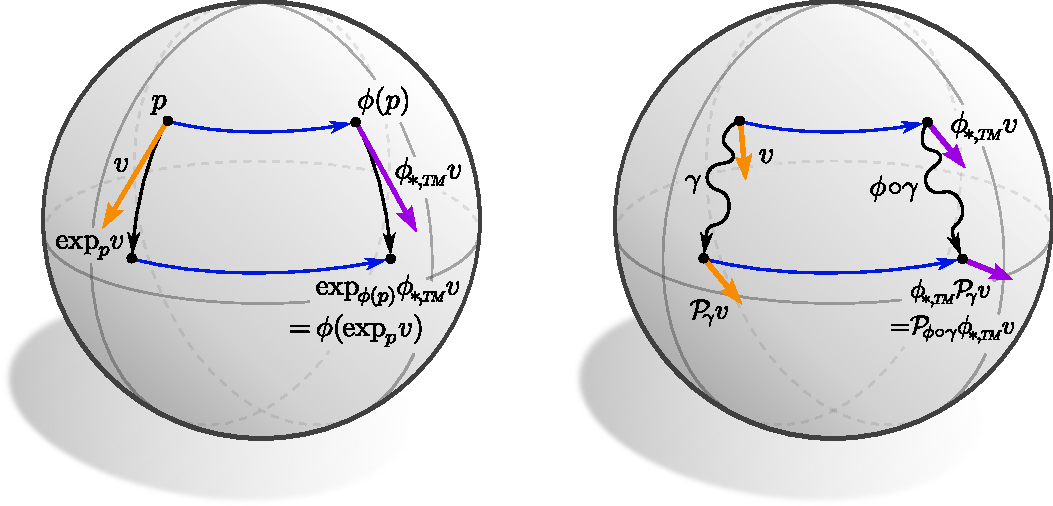
\includegraphics[width=.9\columnwidth]{figures/isometry_exp_transport.pdf}
    \vspace*{1ex}
    \caption{\small
         \emph{چپ:}
        ایزومتری‌ها با نگاشت نمایی جابجا می‌شوند، یعنی،
        $\exp_{\phi(p)} \circ\, \protect\dphiTM (v) \,=\, \phi \circ \exp_p(v)$
        برای هر بردار $v\in \TpM$ و ایزومتری $\phi\in \IsomM$.
         \emph{راست:}
        ایزومتری‌ها همچنین با انتقال لوی-چیویتا بردارهای مماس و بردارهای ویژگی جابجا می‌شوند، یعنی،
        $\protect\dphiA\! \circ \protect\PAgamma \ =\ 
        \mathcal{P}_{\mkern-4mu\overset{}{\protect\scalebox{.6}{$\!\A$}, \mkern1mu\phi\circ\gamma}}\!
        \circ \protect\dphiA$
        برای مسیرهای دلخواه $\gamma:[0,1]\to M$ و ایزومتری‌های $\phi\in \IsomM$.
        اگر یک اتصال جایگزین و \lr{G}-سازگار استفاده شود، ما می‌خواهیم که همان خاصیت جابجایی‌پذیری برای آنها نیز برقرار باشد.
        نامتغیر بودن نگاشت‌های نمایی و منتقل‌کننده‌ها نسبت به ایزومتری به کانولوشن‌های $\GM$ اجازه می‌دهد تا تحت عمل ایزومتری‌ها هم‌متغیر باشند.
    }
    \label{fig:isom_exp_transport}
\end{figure}






\paragraph{ایزومتری‌ها و منتقل‌کننده‌های موازی:}
پیش‌ران روی کلاف مماس در~\cite{gallier2019diffgeom1} علاوه بر این استدلال شد که با منتقل‌کننده‌های متناظر لوی-چیویتا جابجا می‌شود، همانطور که در شکل~\ref{fig:isom_exp_transport} (راست) به تصویر کشیده شده است.
اگر یک اتصال جایگزین و \lr{G}-سازگار برای انتقال بردارهای ویژگی انتخاب شود، ما \emph{می‌خواهیم} که آن نیز با عمل ایزومتری‌ها جابجا شود.
از آنجایی که منتقل‌کننده‌ها و پیش‌ران‌ها بر روی $\FM$، $\GM$ و $\A$ از آنهایی که بر روی $\TM$ هستند القا می‌شوند، می‌توان به راحتی نشان داد که این خاصیت به آنها نیز منتقل می‌شود.
به طور خاص برای کلاف‌های بردار ویژگی الحاقی این به این معنی است که برای ایزومتری‌های دلخواه $\phi \in \IsomGM$ و مسیرهای $\gamma$ ما رابطه
\begin{align}\label{eq:transport_isom_commutation}
    \dphiA\! \circ \PAgamma
    \ =\ 
    \mathcal{P}_{\mkern-4mu\overset{}{\protect\scalebox{.6}{$\!\A$}, \mkern1.5mu\phi \mkern1.5mu\circ\mkern1.5mu \gamma}}\!
    \circ \dphiA
\end{align}
را فرض می‌کنیم، به طوری که نمودار زیر جابجا می‌شود:
\begin{equation}
\quad
\begin{tikzcd}[column sep=70pt, row sep=40, font=\normalsize]
    \A_{\gamma(0)}
        \arrow[r, "\dphiA"]
        \arrow[d, "\PAgamma"']
    &
    \A_{\phi \mkern1mu\circ\mkern1mu \gamma(0)}
        \arrow[d, "\mathcal{P}_{\mkern-4mu\overset{}{\protect\scalebox{.6}{$\!\A$}  \mkern-0mu,\phi \mkern1mu\circ\mkern1mu \gamma}}"]
    \\
    \A_{\gamma(1)}
        \arrow[r, "\dphiA"']
    &
    \A_{\phi \mkern1mu\circ\mkern1mu \gamma(1)}
\end{tikzcd}
\end{equation}






\paragraph{ایزومتری‌ها و پول‌بک‌های منتقل‌کننده میدان‌های ویژگی:}

با دانستن قوانین تبدیل نگاشت‌های نمایی و منتقل‌کننده‌ها تحت عمل ایزومتری‌ها، ما همه چیز لازم را برای استخراج قانون تبدیل پول‌بک‌های منتقل‌کننده $\Expspf$ از میدان‌های ویژگی $f$ در دست داریم:
\begin{thm}[عمل ایزومتری بر روی پول‌بک‌های منتقل‌کننده میدان‌های ویژگی]
\label{thm:transporter_pullback_isometry_action}
    فرض کنید $f\in \Gamma(\A)$ هر میدان ویژگی و $\phi \in \IsomGM$ هر ایزومتری حافظ \lr{G}-ساختار باشد.
    فرض کنید منتقل‌کننده‌های بردار ویژگی با عمل $\IsomGM$ جابجا شوند، یعنی معادله~\eqref{eq:transport_isom_commutation} برقرار باشد
    (که به طور خودکار برای اتصال لوی-چیویتا تضمین می‌شود).
    سپس پول‌بک منتقل‌کننده (تعریف~\ref{dfn:Expf_pullback_field}) از میدان پیش‌ران $\phi\rhd \!f$ (تعریف~\ref{dfn:isometry_pushforward}) به صورت زیر داده می‌شود:
    \begin{align}\label{eq:transporter_pullback_isometry_commutativity}
        \Expsp (\phi \rhd f)
        \ =\ 
        \dphiAout \!\circ \big[\mkern-2mu \Expsphiinvpf \mkern1mu\big] \circ \dphiTM^{-1}
    \end{align}
\end{thm}
\begin{proof}
    ما با اعمال سمت راست بر روی یک بردار دلخواه $v\in\TpM$ شروع می‌کنیم و با استفاده از ویژگی‌های استخراج شده در این بخش به تدریج به سمت چپ می‌رسیم:
    \begin{alignat}{3}
        &\,\ \dphiAout \big[\mkern-2mu \Expsphiinvpf \mkern1mu\big] \, \dphiTM^{-1} (v) \\
        =&\,\ \dphiAout\, \mathcal{P}_{\mkern-5mu\overset{}{\protect\scalebox{.8}{$\!\Ain$},\protect\scalebox{.85}{$\mkern2mu\phiinv(p) \mkern-3mu\leftarrow\mkern-1mu \exp_{\phiinv(p)} \!\circ\mkern2mu \dphiTM^{-1}(v)$}}}
         \circ f \circ \exp_{\phiinv(p)} \mkern-2mu\circ\, \dphiTM^{-1} (v)
            \quad && \big( \text{\small پول‌بک منتقل‌کننده، تعریف~\ref{dfn:Expf_pullback_field} } \big) \notag\\
        =&\,\ \dphiAout\, \mathcal{P}_{\mkern-5mu\overset{}{\protect\scalebox{.8}{$\!\Ain$},\protect\scalebox{.85}{$\mkern2mu\phiinv(p) \mkern-3mu\leftarrow\mkern-1mu \phiinv\mkern-2mu \circ \exp_p (v)$}}}
         \circ f \circ \phiinv \circ \exp_p (v)
            \quad && \big( \text{\small عمل ایزومتری بر $\exp$، معادلۀ~\eqref{eq:exp_isom_commutation}} \big) \notag\\
        =&\,\ \mathcal{P}_{\mkern-5mu\overset{}{\protect\scalebox{.8}{$\!\Ain$},\protect\scalebox{.85}{$\mkern2mu p \mkern-3mu\leftarrow\mkern-1mu \exp_p (v)$}}}
         \circ \dphiAin \circ f \circ \phiinv \circ \exp_p (v)
            \quad && \big( \text{\small عمل ایزومتری بر $\mathcal{P}_{\mkern-5mu\overset{}{\protect\scalebox{.75}{$\!\Ain$}}}$، معادلۀ~\eqref{eq:transport_isom_commutation}} \big) \notag\\
        =&\,\ \mathcal{P}_{\mkern-5mu\overset{}{\protect\scalebox{.8}{$\!\Ain$},\protect\scalebox{.85}{$\mkern2mu p \mkern-3mu\leftarrow\mkern-1mu \exp_p (v)$}}}
         \circ (\phi \rhd f) \circ \exp_p (v)
            \quad && \big( \text{\small پیش‌ران میدان‌ها، معادلۀ~\eqref{eq:pushforward_section_A}} \big) \notag\\
        =&\,\ \big[\mkern-2mu \Expsp (\phi \rhd f) \mkern1mu\big] (v)
            \quad && \big( \text{\small پول‌بک منتقل‌کننده، تعریف~\ref{dfn:Expf_pullback_field} } \big) \notag
    \end{alignat}
\end{proof}
به طور شهودی، این نتیجه فقط بیان می‌کند که پول‌بک منتقل‌کننده یک میدان پیش‌ران برابر با پیش‌ران پول‌بک منتقل‌کننده میدان اصلی است.
نسبت به بدیهی‌سازی‌های محلی، این پیش‌ران را می‌توان به عنوان یک تبدیل پیمانه القا شده از ایزومتری تفسیر کرد، که در معادله~\eqref{eq:transporter_pullback_pushforward_field} بیان شد.
ما در ادامه فرض خواهیم کرد که اتصال \lr{G}-سازگاری که برای انتقال بردارهای ویژگی انتخاب می‌شود، همیشه نسبت به $\IsomGM$ نامتغیر خواهد بود و بنابراین معادله~\eqref{eq:transporter_pullback_isometry_commutativity} برقرار است.


اینکه پول‌بک منتقل‌کننده و پیش‌ران ایزومتری جابجا می‌شوند، نتیجه جابجایی‌پذیری نگاشت نمایی و منتقل‌کننده موازی است، که پول‌بک منتقل‌کننده بر حسب آنها تعریف می‌شود.
توجه داشته باشید که دیفئومورفیسم‌های عمومی متریک و در نتیجه نگاشت نمایی و پول‌بک منتقل‌کننده میدان‌های ویژگی را حفظ نمی‌کنند.
با تکیه بر این ساختارها، تبدیلات میدان کرنل و کانولوشن‌های $\GM$ فقط می‌توانند نسبت به ایزومتری هم‌متغیر باشند اما نه کاملاً نسبت به دیفئومورفیسم.